\documentclass[../main.tex]{subfiles}


\begin{document}
	\section{Základy programování v jazyce Blocky}
	V první kapitole jsme se dozvěděli, jak nastavit naše prostředí tak, abychom mohli začít programovat robota v jazyce Blocky. Tato kapitola se věnuje základním blokům, bez kterých bychom robota programovali jen stěží.

	\subsection{Základní ovládání motorů}
	K ovládání motorů robota budeme pro začátek používat dva základní příkazy (k nalezení v příkazové části, v sekci \textbf{VEX V5 Motors}). Oba slouží k nastavování rychlosti motoru:
	\begin{itemize}
		\blockMotorStart
		\blockMotorStop
	\end{itemize}

	Když robot vykonává náš program a potká tyto dva bloky, tak zapne/vypne daný motor a jde okamžitě na další příkaz. Takovým blokům říkáme neblokující, protože „neblokují“ běh programu.

	K tomu, abychom mohli psát komplexnější programy, budeme potřebovat ještě jeden příkaz, se kterým jsme se setkali v minulé části:
	\begin{itemize}
		\blockWait
	\end{itemize}

	Tento příkaz je blokující -- jakmile na něho při běhu programu dojde, tak musí počkat, než uplyne zadaný čas. Poté se začnou vykonávat bloky pod ním. To mimo jiné znamená, že pokud je to poslední blok programu, tak neudělá nic, protože program ho vykoná a hned poté skončí (už nemá co dalšího vykonávat).

	\begin{question}\label{que:basic}%
		Naprogramujte robota, aby jel dvě vteřiny rovně, otočil se (otáčením doleva/doprava) a poté jel dvě vteřiny dozadu. Nastavte rychlost tak, aby robot jel rozumně rychle.
	\end{question}

	\begin{solution}
		\begin{figure}
			\centering
			\begin{minipage}{0.5\textwidth}
				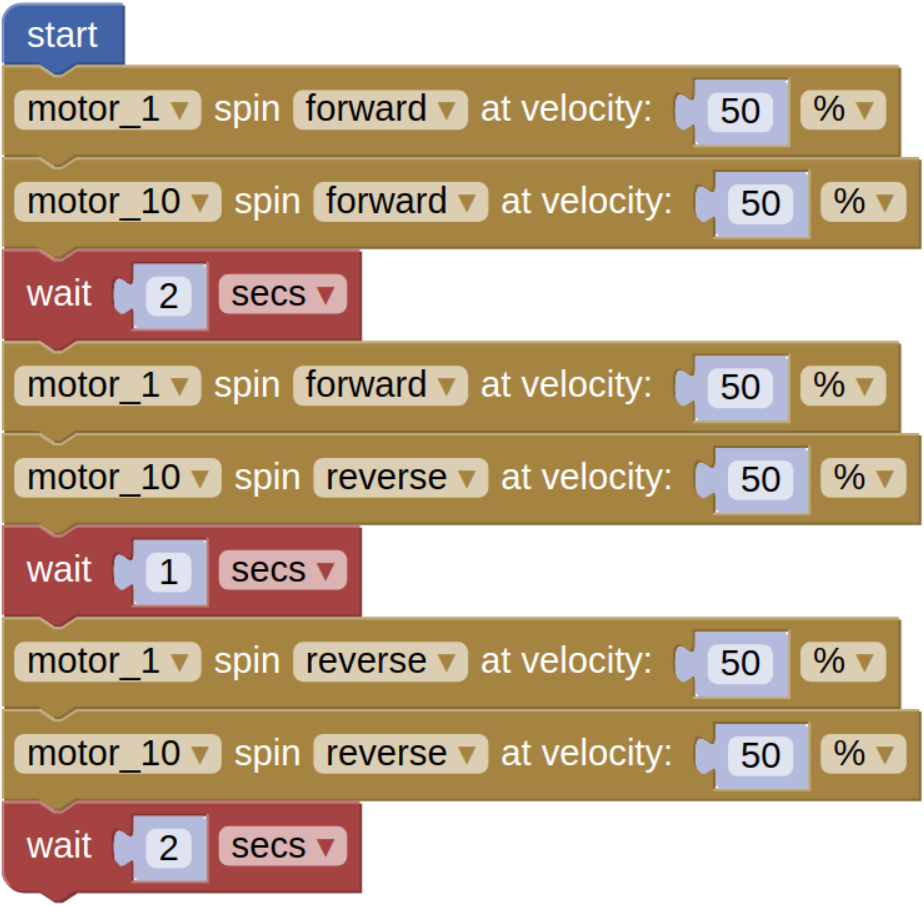
\includegraphics[width=\linewidth]{Images/02/sol2.png}
			\end{minipage}
		\end{figure}
	\end{solution}

	\begin{question}\label{que:loop-example}%
		Naprogramujte robota, aby se „plížil“ -- pomalu jel levým kolem dopředu 1 sekundu a poté pomalu pravým kolem dopředu 1 sekundu. Opakujte dvakrát.
	\end{question}

	\begin{solution}
		\begin{figure}
			\centering
			\begin{minipage}{0.5\textwidth}
				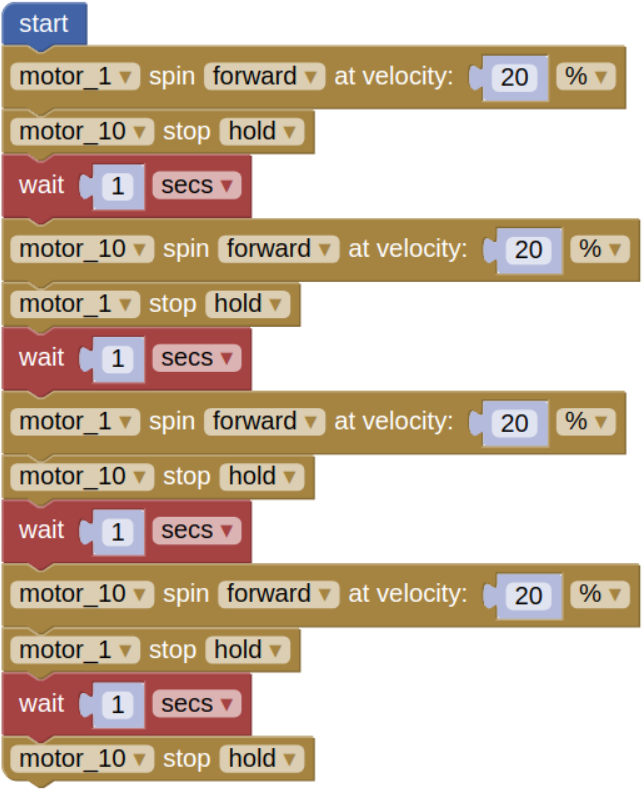
\includegraphics[width=\linewidth]{Images/02/sol3.png}
			\end{minipage}
		\end{figure}
	\end{solution}

	\subsection{Smyčky}
	V příkladu \ref{que:loop-example} jsme několikrát opakovali stejné bloky, což může být pro prográmatora dost nepříjemné. Výrazně jednodušší by bylo, kdybychom mohli prohlásit „opakuj tyto bloky“ -- to je naštěstí přesně, co dělají smyčky.

	Dvě nejzákladnější (k nalezení v příkazové části, v sekci \textbf{Loops}) vypadají takto:
	\begin{itemize}
		\blockLoop
		\blockLoopForever
	\end{itemize}

	\begin{question}
		Upravte příklad \ref{que:loop-example}, aby využíval smyčku. Místo dvakrát opakujte desetkrát.
	\end{question}

	\begin{solution}
		\begin{figure}
			\centering
			\begin{minipage}{0.5\textwidth}
				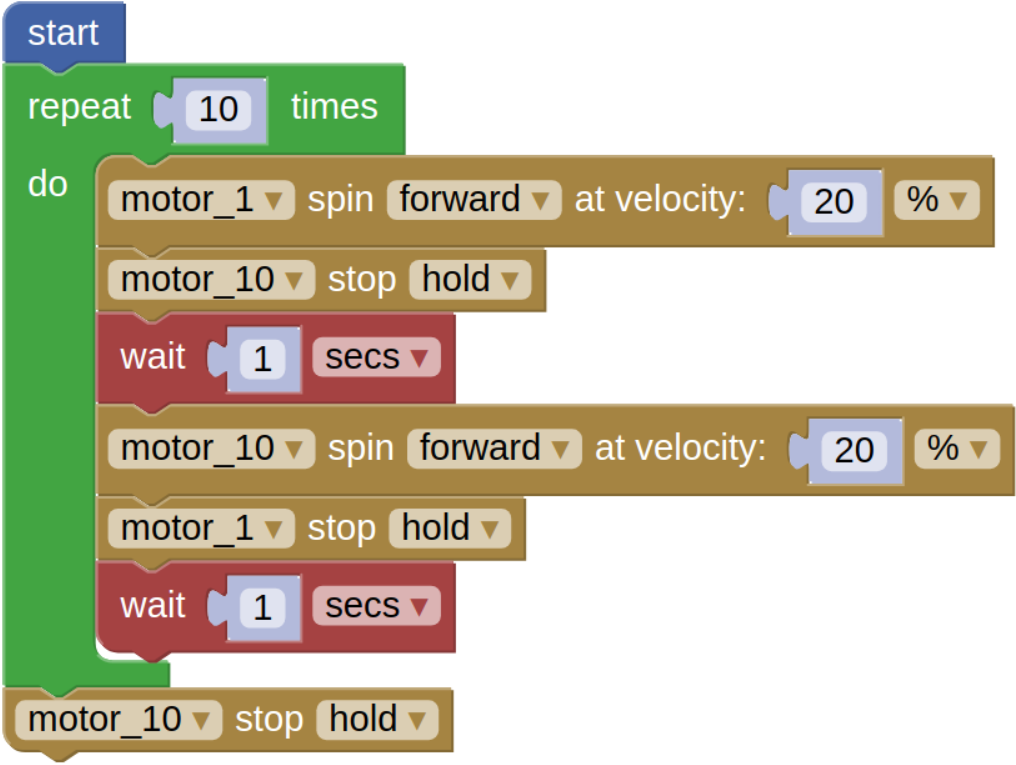
\includegraphics[width=\linewidth]{Images/02/sol4.png}
			\end{minipage}
		\end{figure}
	\end{solution}

	\begin{question}
		Naprogramujte robota, aby donekonečna jezdil do čtverce (1 vteřinu rovně, poté otočení doprava/doleva a opakovat).
	\end{question}

	\begin{solution}
		\begin{figure}
			\centering
			\begin{minipage}{0.5\textwidth}
				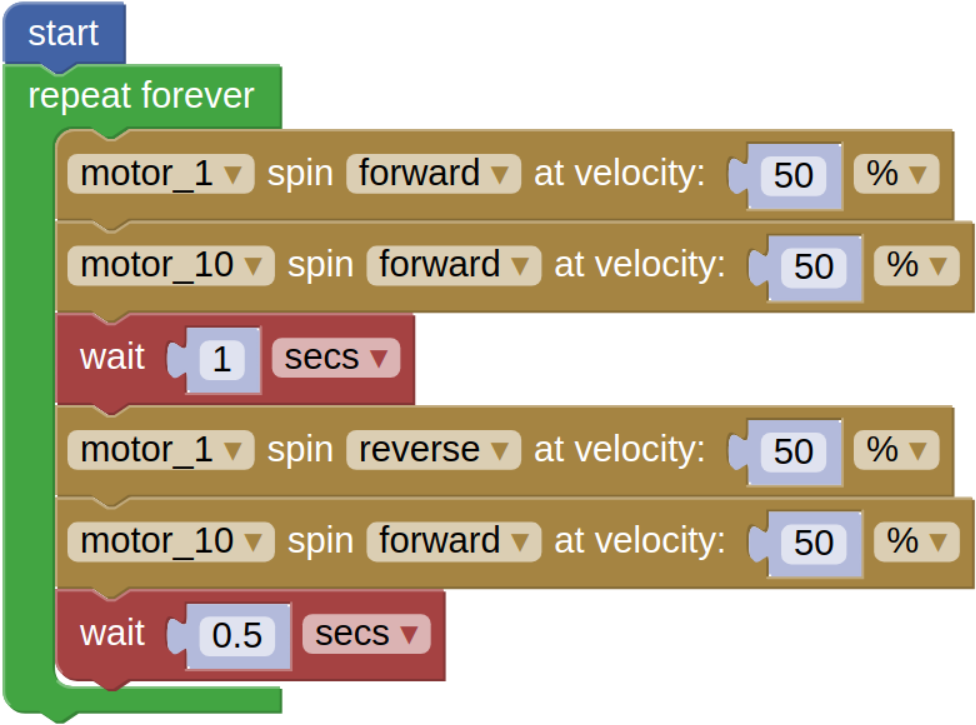
\includegraphics[width=\linewidth]{Images/02/sol5.png}
			\end{minipage}
		\end{figure}
	\end{solution}

	\subsection{Jízda na vzdálenost}\label{cha:distanceride}
	Zatím umíme zapnout daný motor a na nějakou dobu, ale občas by se nám hodilo říct motoru „otoč se o tolik stupňů/otáček.“ Kombinací příkazů motoru a smyček toho můžeme docílit. Budeme k tomu potřebovat následující nové bloky:
	\begin{itemize}
		\blockMotorDistance
		\blockMotorVelocity
		\blockWaitUntil
		\blockMotorDone
	\end{itemize}

	K tomu, aby tedy robot jel rovně 3 otáčky kol, můžeme udělat např. toto:

	\begin{figure}
		\centering
		\begin{minipage}{0.5\textwidth}
			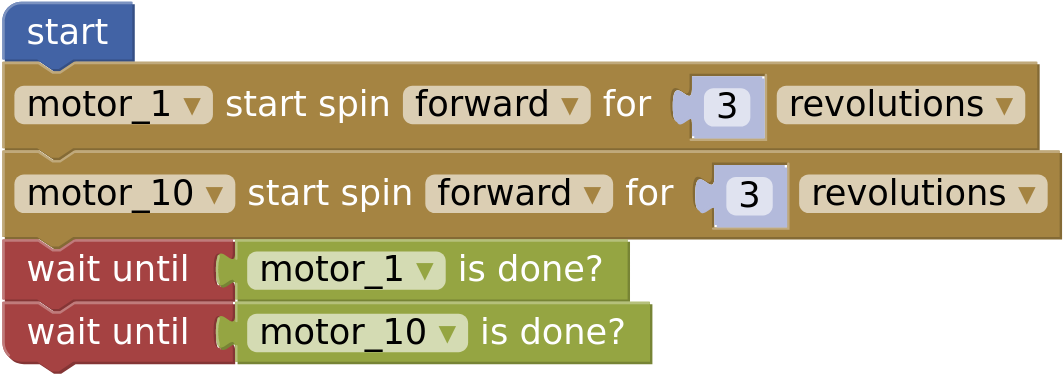
\includegraphics[width=\linewidth]{Images/02/sol.png}
		\end{minipage}
	\end{figure}

	Program nejprve nastaví rychlost motorům a následně je zapne na $3$ otáčky. Poté počká, než oba motory skončí (až se dotočí) a před koncem programu je vypne (což není úplně nutné, ale ničemu neškodí).

	\begin{question}
		Naprogramujte robota, aby jel rovně tři otáčky, otočil se (otáčením doleva/doprava, opět pomocí odhadnutí otáček) a poté jel dvě otáčky dozadu.
	\end{question}

	\begin{solution}
		\begin{figure}
			\centering
			\begin{minipage}{0.45\textwidth}
				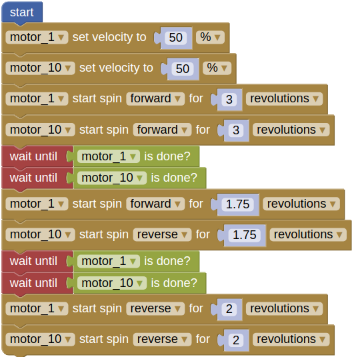
\includegraphics[width=\linewidth]{Images/02/sol6.png}
			\end{minipage}
		\end{figure}
	\end{solution}

	\begin{question*}
		Vytvořte pro robota slalomovou dráhu (např. z ruliček/slepených papírů) a naprogramujte robota, aby jí co nejrychlejí projel a vrátil se zpět do cíle. Bonusové body za to, pokud cestou nepřevrhne ani jednu tyčku.
	\end{question*}

	\subsection{Komentáře}
	Při psaní komplexnější programů je užitečné kód, který není na první pohled přehledný, komentovat. Je to příjemné jak pro ostatní programátory, kteří ho vidí poprvé, tak i pro vás, jako připomenutí (protože po měsíci vám bude připadat, že ho vidíte poprvé).

	Ke psaní komentářů slouží následující blok:
	\begin{itemize}
		\blockComment
	\end{itemize}

	\begin{question}
		Vezměte některý z vašich již vytvořených programů a hezky jej okomentujte.
	\end{question}

\end{document}
